\documentclass[a4paper,12pt]{article}
\usepackage[utf8]{inputenc}
\usepackage[french]{babel}
\usepackage[T1]{fontenc}
\usepackage[top=2cm,bottom=2cm,left=2cm,right=2cm]{geometry}
\usepackage{graphicx}
\usepackage{wrapfig}
\usepackage{url}

\begin{document}

\begin{titlepage}
	\begin{center}
		\Large{Année universitaire 2016-2017}\\
		\Large{Université de Caen Basse-Normandie}\\[1cm]
		
		\huge{Rapport sur le premier semestre}\\
		\vspace{3cm}
		
		Alexis Carreau\\
		Thomas Lécluse\\
		Emma Mauger\\
		Théo Sarrazin\\
		
	\normalsize{\textit{ ~ L2 Informatique}}\\
		\medskip
		\vspace{2cm}
		
	\end{center}
\end{titlepage}

\tableofcontents
\newpage

\section{Introduction}

	\subsection{Présentation}
	Nous avons choisi de réaliser l'IDE (Integrated Developpement Environnement), car nous voulions créer un outil que nous pourrions utiliser par la suite. Ce sujet nous semblais donc intéressant à faire.
	
	Un IDE fournit des facilités au programmeur pour le développement logiciel. Il a pour but de maximiser la productivité du programmeur. Il contient généralement :
	\begin{itemize}
		\item un éditeur de texte, 
		\item un interpréteur, 
		\item un debugger,
		\item un compilateur,
		\item des options avancées comme la recherche de termes, l'autocomplétion, la coloration syntaxique...
	\end{itemize}
	
	Pour notre projet, nous nous inspirons de logiciels déjà existants, tels que Spider, Pycharm, Eclipse ou encore Emacs.
	\begin{figure}[h!]
		\begin{center}
			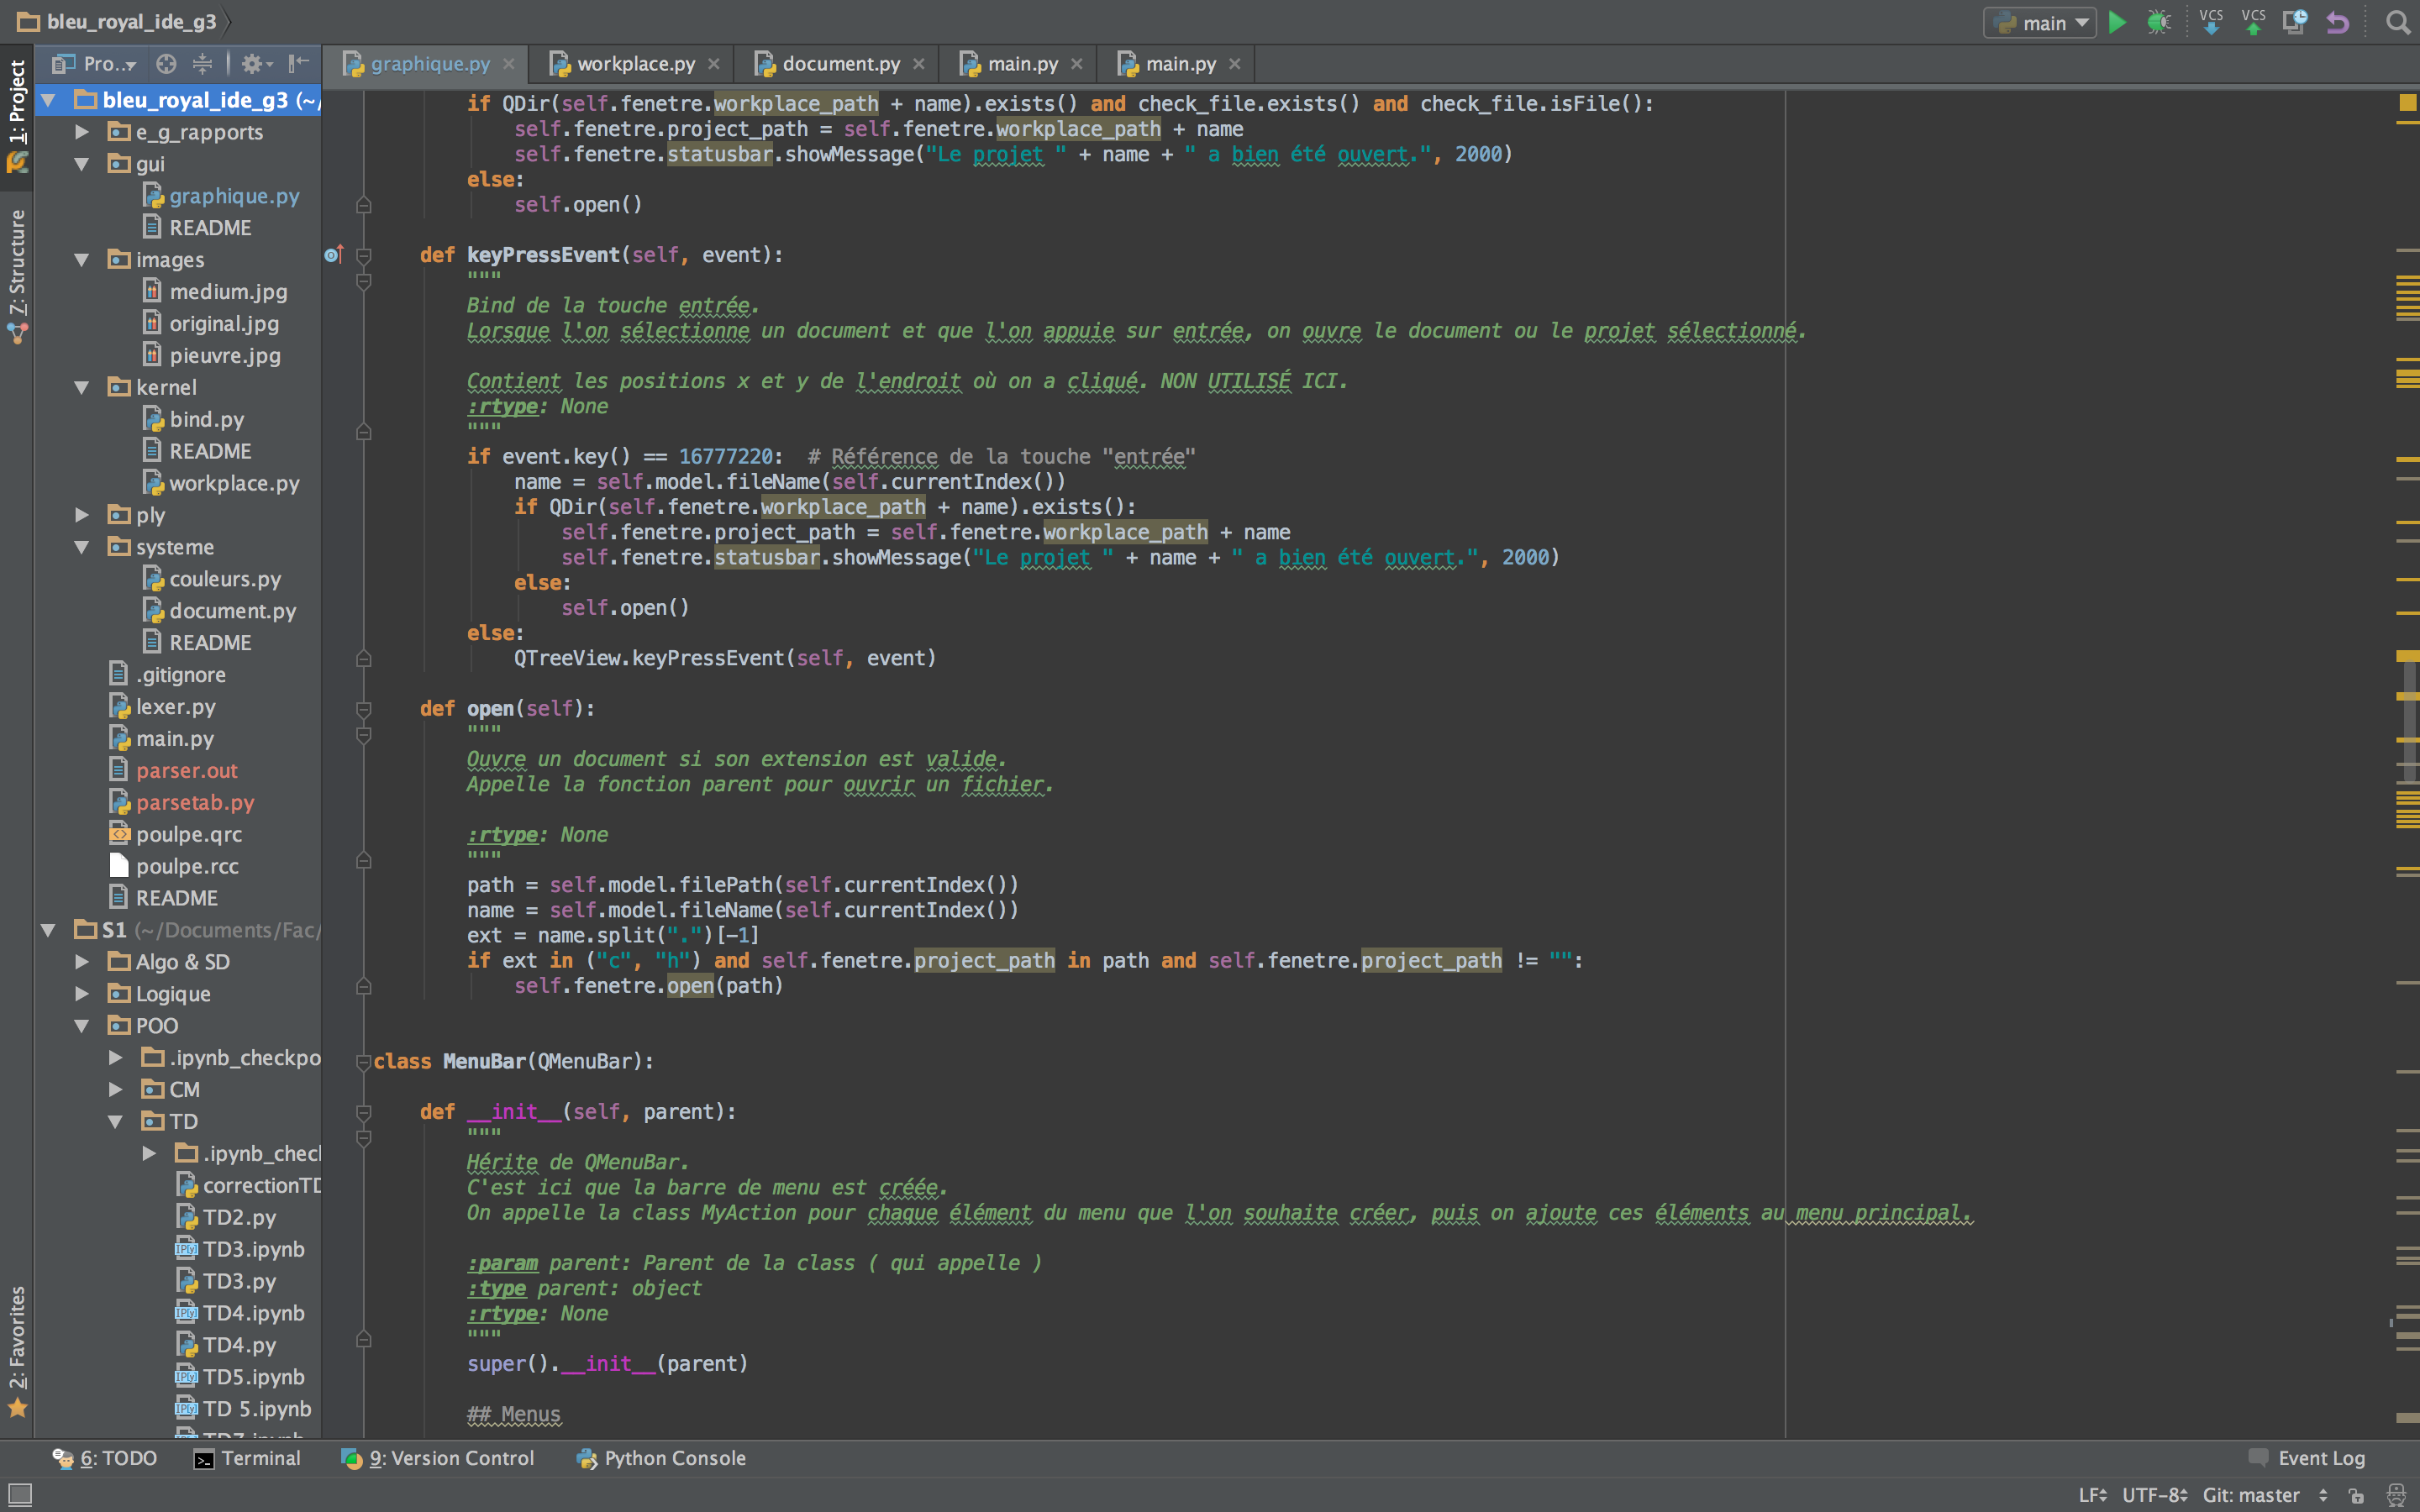
\includegraphics[scale=0.3]{images/pycharm}
			\caption{Exemple d'IDE, ici Pycharm}
		\end{center}
	\end{figure}
	
	\subsection{Objectifs}
	
	Nous devons d'ici à la fin de l'année réaliser un IDE qui contiendra les éléments cités ci-dessus. Pour la coloration lexicale et l'analyse syntaxique du code nous utiliserons les programmes Lex et Yacc.
	
	\subsection{Déroulement et planning}
	
	Nous avons réparti équitablement le travail et le temps de travail de chacun. Il faut préciser que deux membres du groupe (Thomas et Théo) connaissaient déjà la bibliothèque graphique utilisée dans l'IDE, et partaient donc avec un avantage non-négligeable. \\
	Les deux autres membres du groupe ont donc été aidés afin de leur expliquer les bases et de pouvoir démarrer sans trop de problèmes.\\
	
	Nous avons réparti les différentes tâches à effectuer pour le projet entre les membres du groupe. Certaines sont plus longues ou plus complexes, c'est pourquoi certains membres du groupe ont une liste moins remplie que d'autres. Il ne faut donc pas se fier uniquement à cette liste.\\
	
	\begin{itemize}
		\item Alexis : Navigation / Gestion des projets
		\item Emma : Découpage en modules / Architecture projet / Recherche bibliographique / Barre de menu
		\item Théo : Coloration syntaxique / Analyse lexicale / Interface graphique / Gestion (sauvegarde, ouverture) des fichiers
		\item Thomas : Documentation / Interface graphique / Thème, apparence texte et fenêtre / Barre de status
		\item Tout le groupe : Rapports et présentation 
	\end{itemize}
	
\section{Détails techniques}

	\subsection{Bibliothèques utilisées}
	
	Nous avons choisi la bibliothèque graphique QT (version 4.8.7, prévue à la base pour le C++) ce pourquoi nous avons aussi eu besoin de Pyside (version 1.2.4), qui fait le lien vers le langage Python (version 3.4).\\
	
	La raison de ce choix est le fait que QT est un outil puissant de par sa richesse de fonctionnalités. Sa documentation est de plus très fournie car les utilisateurs de QT sont plus nombreux que ceux de Tkinter par exemple.
	
	\subsection{Techniques et logiciels employées}
	
	Nous programmons en python, car c'est un langage qui est multi-plateforme, il plutôt simple et permet de faire vraiment beaucoup de choses. De plus, se documenter est facile car beaucoup de gens l'utilisent, il existe donc plusieurs sites où l'on peut trouver des réponses en cas de problème (stackoverflow, openclassroom...).
	
	Nous avons choisi un style de programmation orienté objet, puisque plus logique dans un projet de cette envergure. L'objet nous permet de mettre en application les notions vues en cours. Cela nous permet de personnaliser en les ré-implémentant des classes de QT pour les adapter à nos besoins.\\
	
	Lex est un programme qui permet de reconnaître des tokens qui sont des éléments d'une chaîne de caractères. Cela à l'aide de règles lexicales que l'on lui passe en entrée.\\
	Dans notre cas, nous utilisons Lex pour reconnaître les éléments que l'on écrit, afin de colorier ces derniers en fonction de leur rôle (identifiant, entier, déclaration...). Nous utilisons la sortie générée en la passant à un autre programme : Yacc.\\
	
	Yacc permet de générer un arbre syntaxique abstrait qui nous permet de vérifier que la syntaxe de notre code est correcte. Aussi, cela permet de proposer une complétion automatique en fonction de ce que l'on écrit.\\
	Nous devons également lui passer des règles, qui sont d'ordre grammaticales.
	
	\begin{figure}[h!]
		\begin{center}
			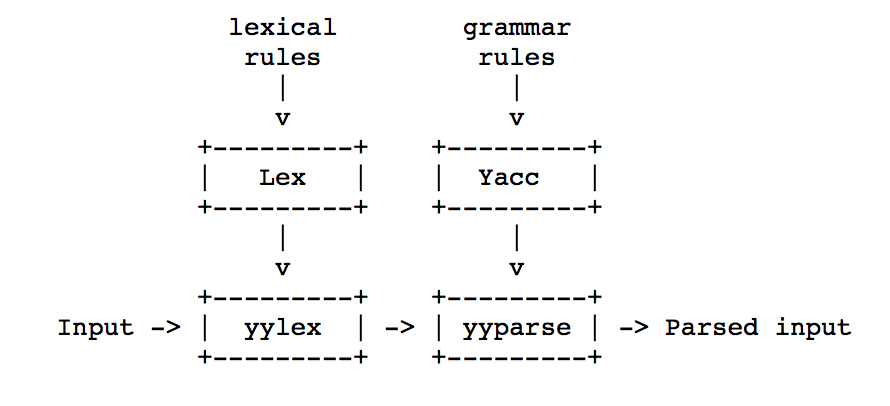
\includegraphics[scale=0.7]{images/schema_lex_yacc}
			\caption{Schéma résumant le fonctionnement de Lex et Yacc.}
		\end{center}
	\end{figure}
	
	\subsection{Bibliographie}
	
	Nous avons utilisé deux sites de documentation principalement sur QT et Pyside.
	\begin{itemize}
		\item \url{http://srinikom.github.io/pyside-docs/PySide/QtGui/}
		\item \url{doc.qt.io}
	\end{itemize}
	
\section{Structure générale}

	\subsection{Répartition en modules}
	
		Les différents modules sont répartis par thèmes. Nous avons :
		\begin{itemize}
			\item Un module pour l'interface graphique
			\item Un module pour la gestion des évènements
			\item Un module pour la gestion des fichiers
			\item Un module pour la gestion des projets
			\item Un module pour la coloration syntaxique (avec Lex)
		\end{itemize}
	
	\subsection{Module graphique}
	
		On retrouve dans ce module tout ce qui est relatif au GUI (l'interface graphique).\\
		C'est là qu'est créée la fenêtre principale de l'application, où l'on va pouvoir créer, ouvrir, sauvegarder des fichiers et des projets.\\
		Nous n'hésitons pas à créer des classes afin de modifier les objets de QT pour les adapter en fonction de nos besoins. Cela permet aussi dans certains cas de compacter le code.
		On retrouve dans ce module ce qui est nécessaire pour :
	
			\subsubsection*{Créer une zone de texte}
			 Nous utilisons pour cela l'objet QTextEdit de QT, qui est un widget permettant d'avoir une zone de texte. Nous nous en servons comme fenêtre d'éditeur, c'est donc ici que l'on pourra écrire du code.\\
			Le thème de l'application, (c'est à dire la couleur de fond et de la police ainsi que cette dernière) est relatif au QTextEdit. C'est également là que la couleur des éléments (tokens) sera modifiée par Lex en fonction de leur rôle.\\
			\begin{center}
				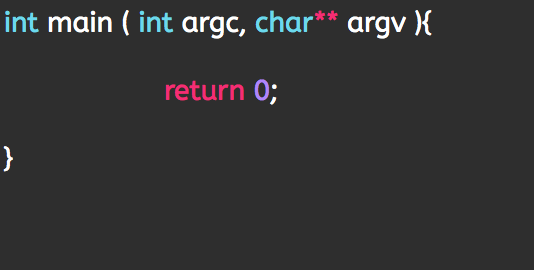
\includegraphics[scale=1]{images/QTextEdit}
				\vspace{0.5cm}
			\end{center}
			Nous avons ici une classe "Editeur" qui hérite de cet objet. Cela nous permet de paramétrer (couleurs, police et taille d'écriture) la zone de texte afin de pouvoir la créer plus facilement.\\
			
			
			\subsubsection*{Créer plusieurs onglets de code}
			 C'est un QTabWidget que nous utilisons pour cela. Il va créer plusieurs QTextEdit (ou en supprimer si on ferme l'onglet), et possède des fonctions et raccourcis pour naviguer entre tous. \\
			Si aucun onglet n'est ouvert, le logo de notre groupe est affiché à la place.\\
			\begin{center}
				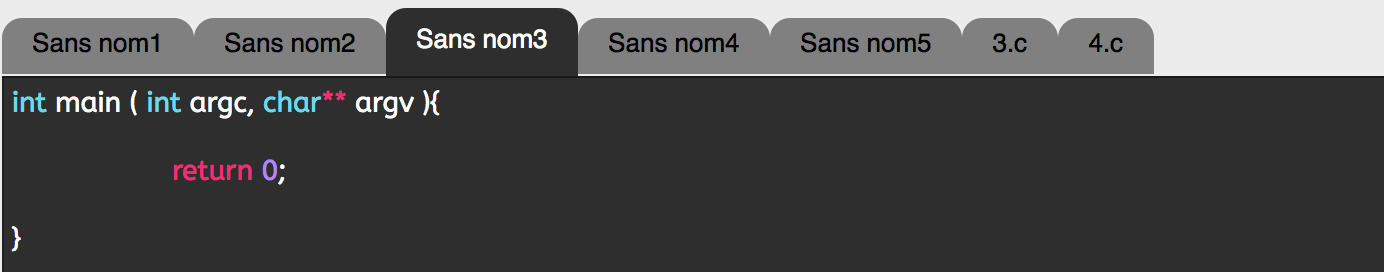
\includegraphics[scale=0.6]{images/QTabWidget}
				\vspace{0.5cm}
			\end{center}
			Nous avons créé une classe "TabWidget" qui hérite de cet objet. Un onglet est en fait un QTextEdit, nous créons donc une nouvelle instance de notre classe "Editeur" pour chaque onglet. Le style des onglets, ainsi que le logo du groupe sont mis en place dans cette classe. On utilise pour cela des stylesheets de CSS.\\
			
			
			\subsubsection*{Créer une barre de menu}
			 Cela permet d'avoir toutes les fonctionnalités et éventuellement des raccourcis. On utilise une QMenuBar pour cela, qui va elle-même utiliser une QAction pour créer une action sur le menu. Une action contient un nom, éventuellement un raccourci et une fonction à exécuter. \\
			\begin{center}
				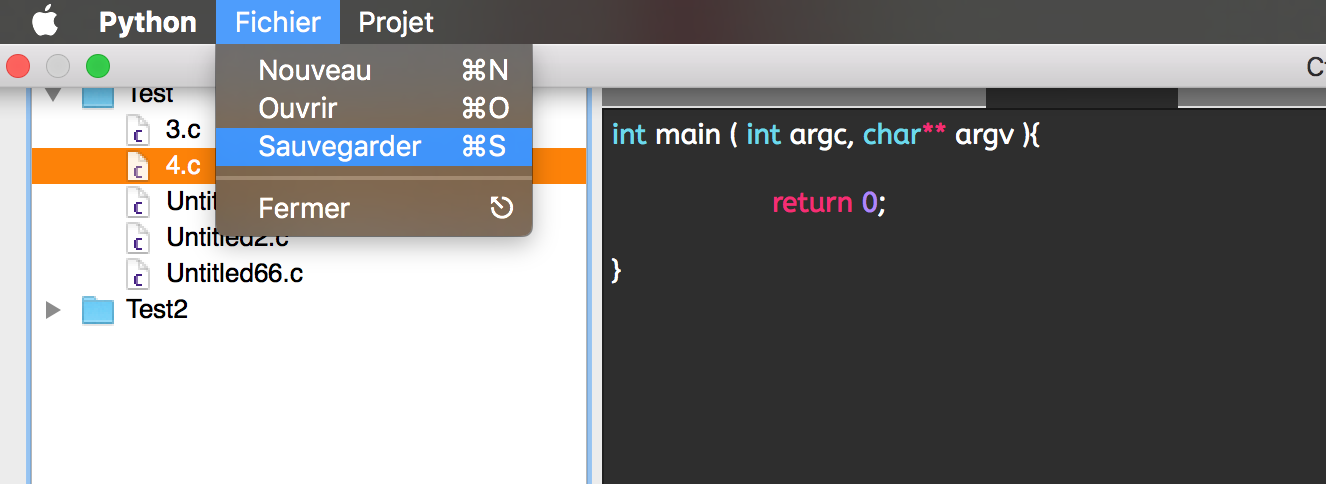
\includegraphics[scale=0.6]{images/QMenuBar}
				\vspace{0.5cm}
			\end{center}
			Nous avons ici deux classes. La première, "MyAction" hérite de QAction et permet tout simplement d'initialiser une action avec son nom, éventuellement un raccourci et une fonction à exécuter. Cela permet de compacter la création d'onglets dans notre menu.\\
			Ensuite nous avons une classe "MenuBar" qui hérite de QMenuBar et qui va créer toutes les instances de MyAction nécessaires à la créations des sous-menus et des onglets du menu. Les actions sont ensuite ajoutées aux menus.\\
			
			
			\subsubsection*{Mettre en place le navigateur de fichiers et de projets}
			 Nous utilisons un QTreeView et un modèle QFileSystemModel qui nous permet d'afficher l'arborescence des fichiers et projets. C'est ce que l'on utilise pour ouvrir et naviguer dans les projets ouverts.\\
			\begin{center}
				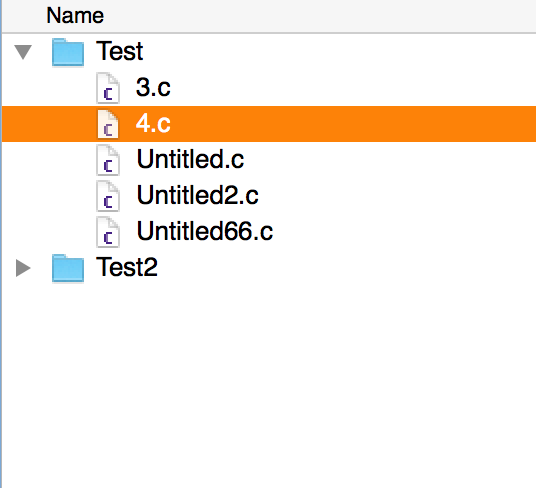
\includegraphics[scale=0.6]{images/QTreeView}
				\vspace{0.6cm}
			\end{center}
			Notre classe "TreeView" hérite de QTreeView et permet d'instancier correctement le navigateur. Par exemple pour lui demander de filtrer les fichiers pour n'afficher que les fichiers en .c et .h. On créée aussi des méthodes pour pouvoir ouvrir des projets et des fichiers en double-cliquant dessus mais elles sont placées dans un autre module.\\			
			
			
			\subsubsection*{Modifier la taille du navigateur de fichier/de l'éditeur de code}
			Pour cela, nous utilisons un QSplitter.\\ 
			Cela peut permettre, en fonction de la taille du projet et des répertoires imbriqués dans d'autres, de visualiser complètement les fichiers. Au contraire, on peut réduire le navigateur de fichier pour avoir une zone de code plus grande.\\
			\begin{center}
				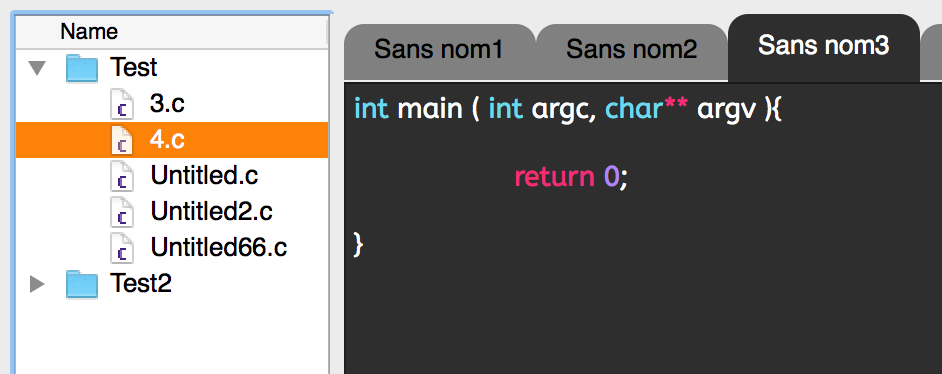
\includegraphics[scale=0.6]{images/QSplitter_1}
				\vspace{0.6cm}
			\end{center}

			\begin{center}
				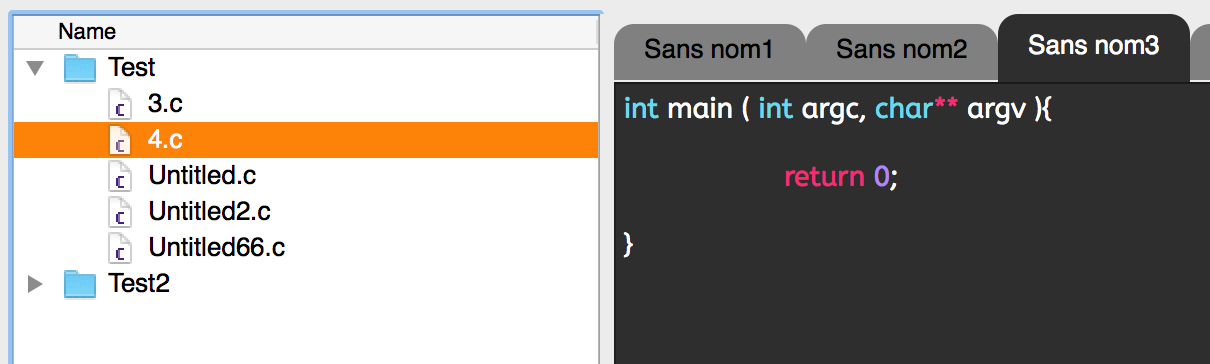
\includegraphics[scale=0.6]{images/QSplitter_2}
				\vspace{0.6cm}
			\end{center}
			Le QSplitter ne nécessite pas de modifcations particulières. En fait on créé juste un objet QSplitter, Et on ajoute les widgets de notre choix dedans. Ils seront donc dans une sorte de boîte dont on peut changer la taille.\\
			
			
			\subsubsection*{Afficher une barre de status}
			 Cela peut être pratique pour afficher des messages sans pour autant utiliser une popup. On y affiche généralement des informations (la plupart temporairement) comme la sauvegarde réussie d'un fichier, l'ouverture d'un projet, le nombre de lignes... L'objet QT qui permet cela est une QStatusBar et nous avons choisi de la placer tout en bas de l'application.\\
			\begin{center}
				
\includegraphics[scale=0.6]{images/QStatusBar}
				\vspace{0.6cm}
			\end{center}
			De même que pour le QSplitter, pour l'usage que nous en avons, il n'est pas nécessaire de faire une classe qui hérite de QStatusBar. Il suffit juste de la créer et d'afficher des messages avec une méthode.\\
			
			
			\subsubsection*{Créer la fenêtre principale}
			Nous utilisons un QWidget, qui est en fait une sorte de parent de tous les objets cités ci-dessus. Nous avons une classe "Fenetre" qui hérite de cet objet. C'est ici que l'on instancie tout les objets précendemment cités.\\
			\begin{center}
				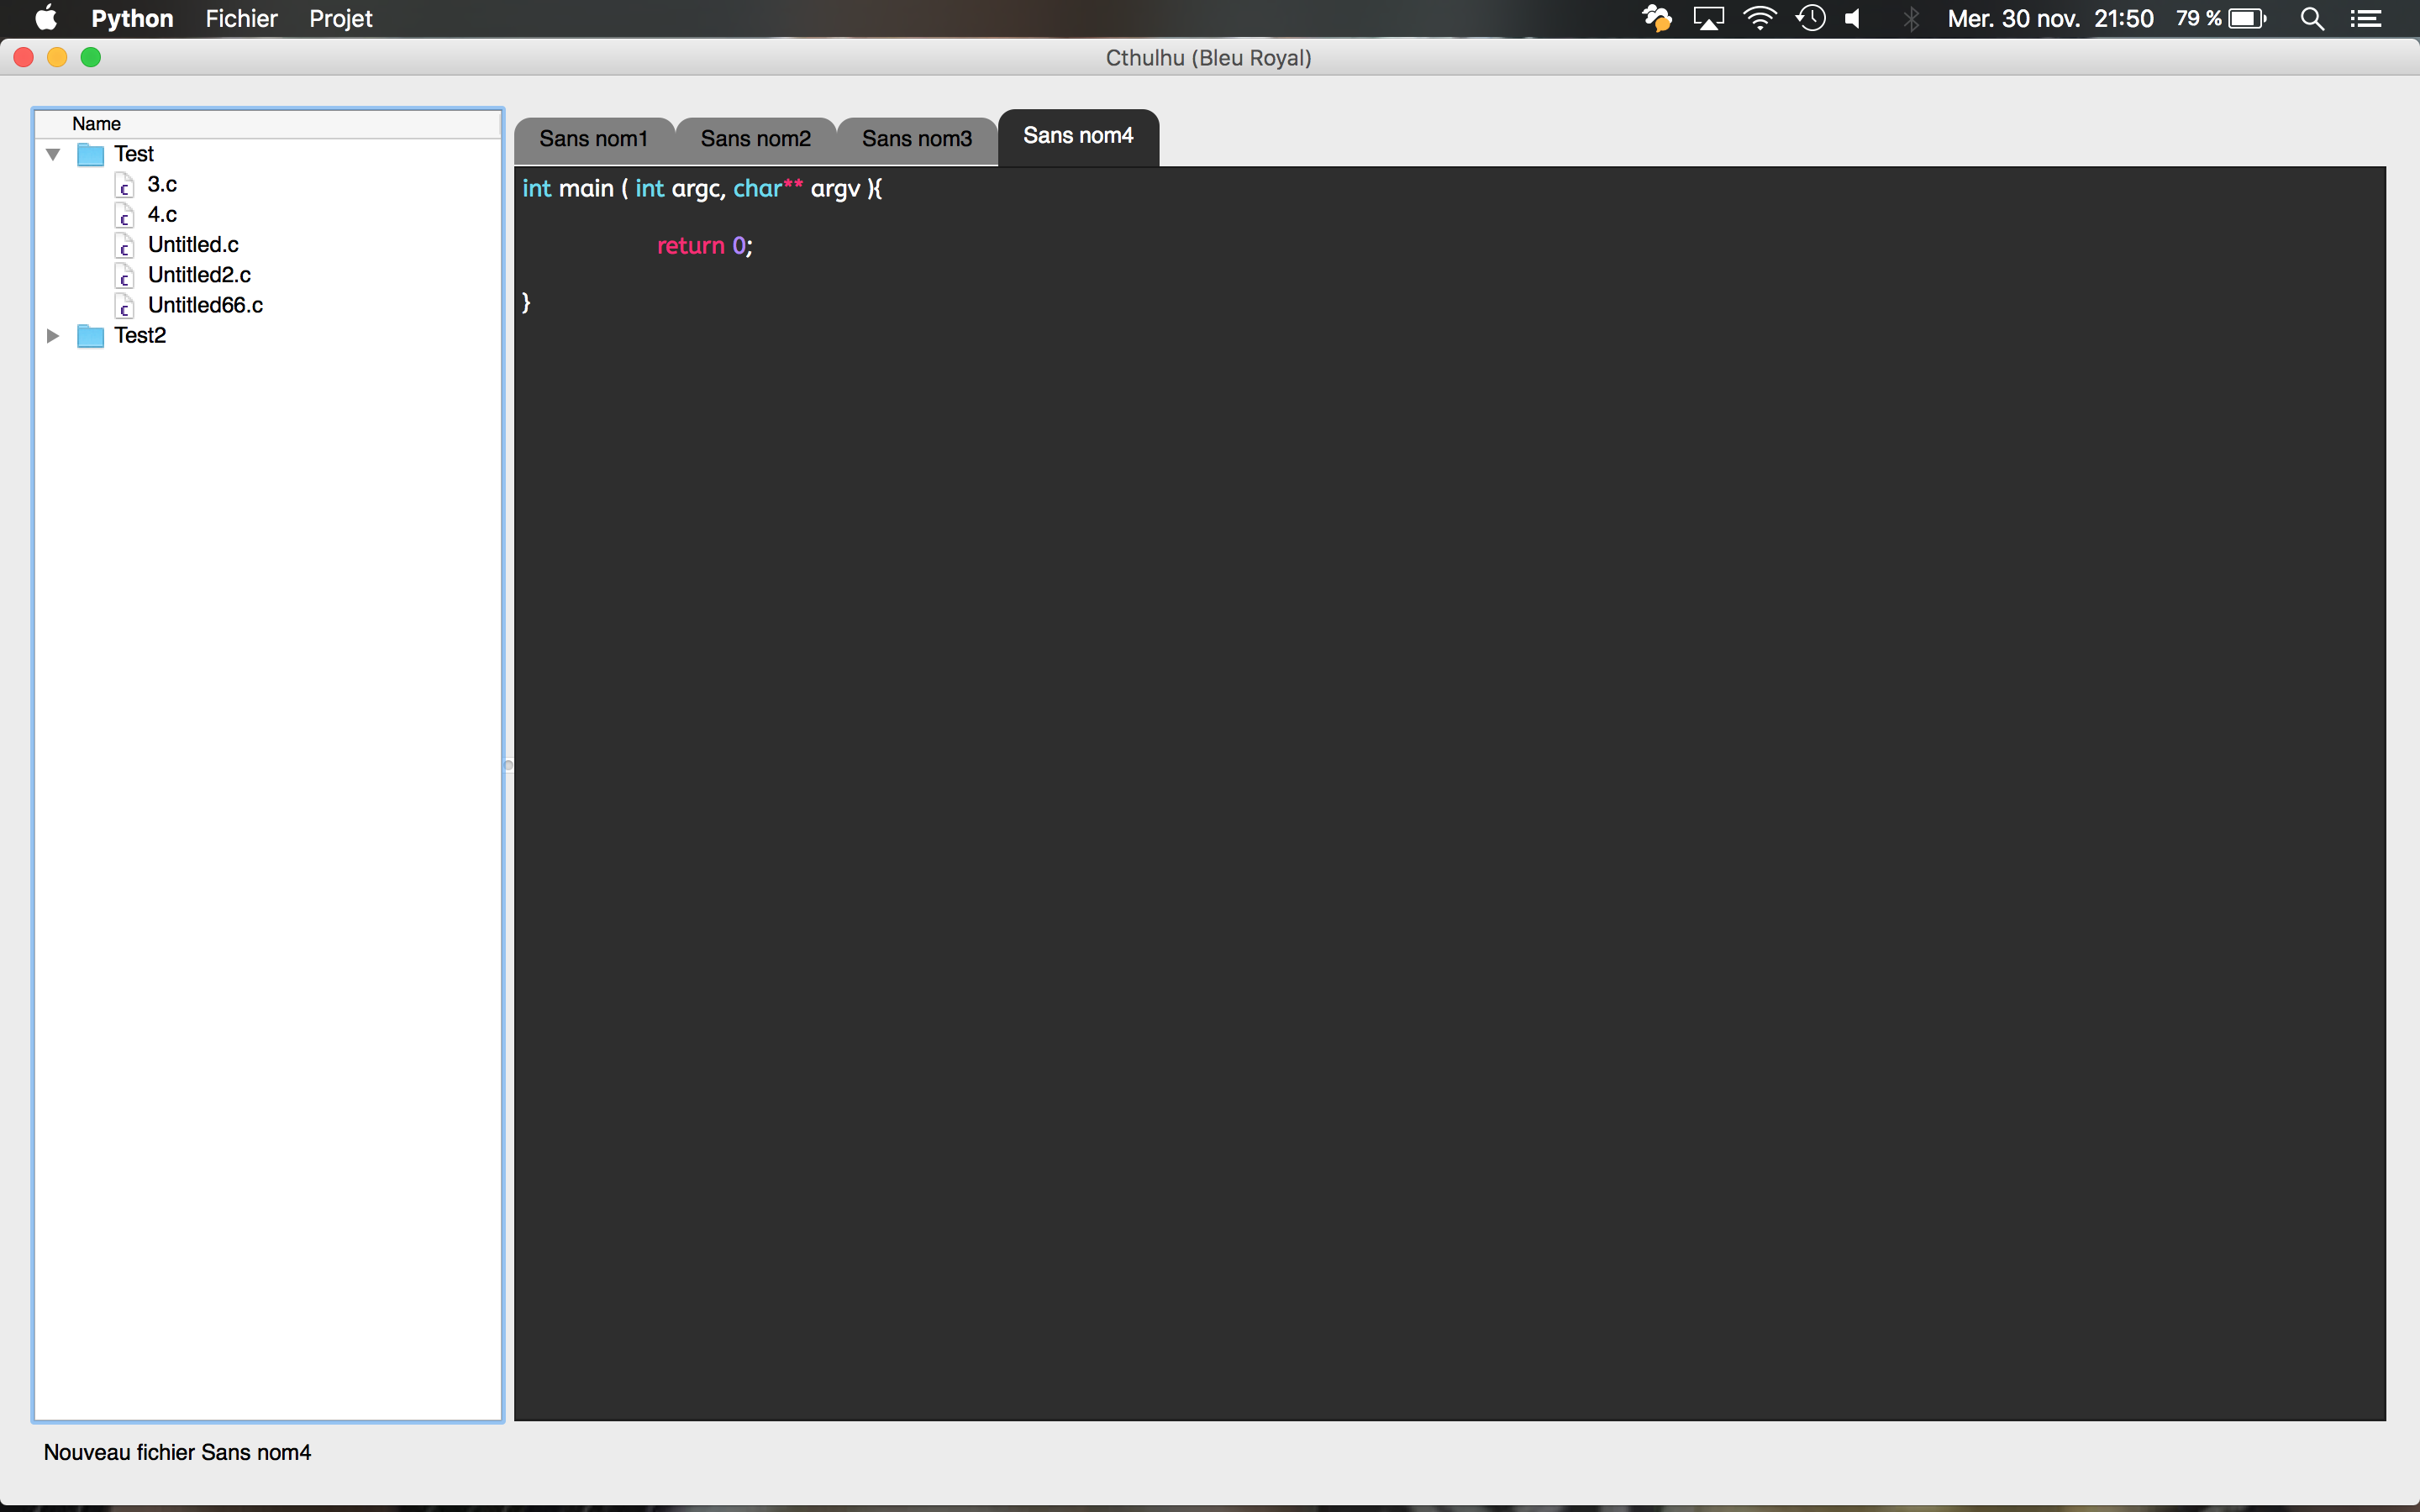
\includegraphics[scale=0.2]{images/QWidget}
				\vspace{0.6cm}
			\end{center}
			
			
			\subsubsection*{Shéma UML récapitulatif}
					
					================ ICI UML ================
		
		\subsection{Module gestion des évènements}
		
		\subsection{Module gestion des fichiers}
		
		\subsection{Module gestion des projets}
		
		Dans un IDE, la présence d’un navigateur de fichier s’impose afin d’avoir un certain confort pour parcourir l’arborescence de projets constitués de programmes (de fichiers). Qui dit projets, dit dossiers, dit fichiers, il faut donc afficher ce contenu dans le navigateur de fichiers. Pour intégrer ce dernier dans notre IDE, nous avons utilisé la classe QTreeview et comme modèle QFileSystemModel et nous avons mis en place un filtre afin de naviguer seulement avec des fichiers C et H. La gestion des projets se fait avec un système Workplace, c’est-à-dire que les projets sont crées dans un dossier Workplace à la racine de l’ordinateur. Un fichier de configuration .xml est ajouté automatiquement dans chaque projet, donc dans chaque dossier, lors de sa création afin d’interdire certaines conditions, par exemple la création d’un projet en dehors de l’IDE donc directement dans le dossier Workplace. Dans l’IDE, pour ouvrir un projet et un fichier, il faut cliquer deux fois sur ce dernier ou appuyer sur entrée ou alors directement avec les boutons ouvrir du menu. Il est également possible de créer un projet ou un fichier, de le sauvegarder, de le fermer ou encore de le supprimer avec les boutons prévus à cet effet dans le menu et les raccourcis clavier. 
Une barre d’état permet de rendre compte, via l’affichage de messages, de ces différentes situations (avec la classe QStatusBar). 
Nous avons également créer une fonction permettant de cacher les dossiers \_\_pycache\_\_ et leur contenu en les supprimant à l'exécution du programme, notamment afin de ne pas les voir dans le navigateur de fichiers ainsi donc que dans le dossier d’exécution de l’IDE, mais maintenant que les projets et les fichiers sont créé dans le dossier Workplace, à la racine de l’ordinateur donc, il n’y a plus de dossier \_\_pycache\_\_ mais cette fonction sert donc encore pour le dossier d’exécution. Cette fonction a été réalisée en maniant des outils système tels que os et shutil.

			\subsubsection*{Créer un nouveau projet}
			Nous utilisons une fonction new\_project dans le module projets. Cette dernière s'assure que le projet créé a un nom différent d'un projet déjà existant, et qu'il ne comporte pas de "/" dans son nom. \newpage Tant que ces conditions ne sont pas respectées la fonction demande un nom de projet.\\
			
			\subsubsection*{Ouvrir un projet}
			Nous utilisons une fonction open\_project dans le module projets. Cette dernière parcours tous les projets existants et si le projet sélectionné est bien un dossier (contenant un .xml), elle l'ouvre.\\
			
			\subsubsection*{Fermer un projet}
			Nous utilisons une fonction close\_project dans le module projets. Cette dernière réinitialise différentes variables afin de revenir à la configuration initiale, comme si nous venions d'ouvrir l'IDE.\\
			
			\subsubsection*{Supprimer un projet}
			Nous utilisons une fonction delete\_project dans le module projets. Cette dernière ....\\
			
		\subsection{Module coloration syntaxique}	
	
\section{Conclusion}
	
	\subsection{Améliorations}
	Il nous reste à intégrer Yacc à notre IDE au second semestre. Mais nous allons aussi :
	\begin{itemize}
			\item Gérer la fermeture de l'IDE lorsque le document n'a pas été sauvegardé
			\item Numéroter les lignes de l'éditeur de texte
			\item Intégrer le nombre de lignes à la barre de statut
			\item Intégrer des boutons de paramètres dans le menu et l'IDE afin de personnaliser ce dernier, par exemple changer le thème.
			\item Gérer la suppression des projets et des fichiers directement depuis l'IDE
			\item Gérer la fermeture des fichiers 
			\item Ajouter un débugger
			\item Ajouter un compilateur
			\item Ajouter l'auto-complétion
			\item Ajouter l'indentation automatique
	\end{itemize}
\end{document}